\documentclass[10pt,a4paper]{article}
\usepackage[utf8]{inputenc}
\usepackage{amsmath}

\makeatletter
\ams@newcommand{\iiiiint}{\DOTSI\protect\MultiIntegral{5}}
\renewcommand{\MultiIntegral}[1]{%
  \edef\ints@c{\noexpand\intop
    \ifnum#1=\z@\noexpand\intdots@\else\noexpand\intkern@\fi
    \ifnum#1>\tw@\noexpand\intop\noexpand\intkern@\fi
    \ifnum#1>\thr@@\noexpand\intop\noexpand\intkern@\fi
    \ifnum#1>4 \noexpand\intop\noexpand\intkern@\fi % <---- added

    \noexpand\intop
    \noexpand\ilimits@
  }%
  \futurelet\@let@token\ints@a
}
\makeatother

\makeatletter
\ams@newcommand{\iiiiiint}{\DOTSI\protect\MultiIntegral{6}}
\renewcommand{\MultiIntegral}[1]{%
  \edef\ints@c{\noexpand\intop
    \ifnum#1=\z@\noexpand\intdots@\else\noexpand\intkern@\fi
    \ifnum#1>\tw@\noexpand\intop\noexpand\intkern@\fi
    \ifnum#1>\thr@@\noexpand\intop\noexpand\intkern@\fi
    \ifnum#1>4 \noexpand\intop\noexpand\intkern@\fi % <---- added
	\ifnum#1>5 \noexpand\intop\noexpand\intkern@\fi % <---- added
    \noexpand\intop
    \noexpand\ilimits@
  }%
  \futurelet\@let@token\ints@a
}
\makeatother

\usepackage{braket}

\newcommand{\RomanNumeralCaps}[1]
    {\MakeUppercase{\romannumeral #1}}
\usepackage{amsfonts}
\usepackage{amssymb}
\usepackage{float}
\usepackage{verbatim}
\usepackage{listings}
\usepackage{hyperref}

\usepackage{pbox}

%bibliography packages, bibliography files are plain text files marked .bib 
%... in the same directory as the .tex file.
\usepackage[nottoc,numbib]{tocbibind}
\usepackage{cite}

\usepackage{color} %red, green, blue, yellow, cyan, magenta, black, white
\definecolor{mygreen}{RGB}{28,172,0} % color values Red, Green, Blue
\definecolor{mylilas}{RGB}{170,55,241}
\usepackage{amsmath}
\usepackage{graphicx}
\graphicspath{{C:/Users/adria/Pictures/FYS3150/}} 
\author{Adrian Martinsen Kleven, Simon Schrader}
\title{Project 3}

\lstset{
 	language =C++,   
    frame=tb, % draw a frame at the top and bottom of the code block
    tabsize=4, % tab space width
    showstringspaces=false, % don't mark spaces in strings
    numbers=left, % display line numbers on the left
    commentstyle=\color{green}, % comment color
    keywordstyle=\color{blue}, % keyword color
    stringstyle=\color{red} % string color
}

\begin{document}

\part*{-Project 3 - FYS3150/FYS4150-
}
{\large By Simon Schrader (4150), Adrian Kleven (3150) - autumn 2019
}
\tableofcontents

\listoffigures
\listoftables
\clearpage
 
\section{Abstract}
Determining the ground state correlation energy between two electrons in a helium atom can be done by evaluating a certain six- dimensional integral assuming that the electrons can be modelled separately, as two, single- particle wave functions of an electron in the hydrogen atom \cite{Problem_set_3}. This integral is also applicable in other aspects of quantum mechanics \cite{Problem_set_3}. For this reason, it's of great value to examine different approaches to solving such integrals, as well as those with higher degrees of freedom. To solve this integral, two different approaches relying on Gaussian quadrature and Monte- Carlo integration were used, as well as the implementation of parallelization to speed up the programs.\\\\Solely using Gauss- Legendre quadrature was found to be poor choice for this application as it's most applicable on finite intervals, however after a change of variables, using both Gauss- Legendre and Gauss- Laguerre quadrature gave good results.\\Both implementations of Monte- Carlo integration however, proved to be a lot more effective than Gaussian quadrature both in accuracy and time expenditure (see figure \ref{Error_time_use}). Especially when using importance sampling did the Monte- Carlo integration see a marked increase in accuracy with fewer mesh points.\\The addition of parallel computing sped the process up by over $350\%$ given $10^7$ mesh points. See figure \ref{N vs. relative time use}.
\section{Introduction} 
The purpose of this article is to apply different versions of Gaussian quadrature and Monte- Carlo integration in solving a six- dimensional integral to examine their times expenditure and accuracy, as well as the effect of parallelizing the C++ implementations of these methods.\\\\Gauss- Legendre and Gauss- Laguerre quadrature takes advantage of two different sets of polynomials, orthogonal under some inner product, and applicable on two different types of intervals. By applying either the Gauss- Legendre quadrature or the Gauss- Laguerre quadrature to the integral (possibly after some change of variables or coordinate system), it's possible to benchmark each of their respective accuracies with the analytical result of the integral as well as compare their time expenditure.\\\\In addition, this article will examine the effectiveness of importance sampling in Monte- Carlo integration, its impact on time expenditure and how much faster it converges towards the real value.
\section{Methods}
The expectation value of the correlation energy between two electrons interacting under the Coulomb interacting is given by the integral
\begin{equation}\label{eq:correlationenergy}
   \langle \frac{1}{|{\bf r}_1-{\bf r}_2|} \rangle =
   \int_{-\infty}^{\infty} d{\bf r}_1d{\bf r}_2  e^{-2\alpha (r_1+r_2)}\frac{1}{|{\bf r}_1-{\bf r}_2|}.
\end{equation}
where 
$$
   {\bf r}_i =  x_i {\bf e}_x + y_i {\bf e}_y +z_i {\bf e}_z
$$
and
$$
r_i = \sqrt{x_i^2+y_i^2+z_i^2}.
$$
$\alpha = 2$, corresponding to the charge of the nucleus of the helium atom as given by \cite{Problem_set_3}.
\subsection{Gaussian quadrature}\label{Gaussian quadrature}
The method of Gaussian quadrature allows one to approximate a function $f(x)$ with a polynomial $P_{2N-1}(x)$ of degree $2n-1$, using only $N$ mesh points. Said polynomial is constructed using sets of orthogonal polynomials, meaning they have the property that
\begin{equation}
\int_a^b P_i(x)P_j(x)W(x)dx = C_{ij}\delta_{ij}
\end{equation}
where $\big\{ P_k\hspace{1mm}|\hspace{1mm} k \in \mathbb N \big\}$ is the set of polynomials orthogonal in the domain $[a,b]$, $\delta_{ij}$ is the Kronecker- delta and $P_0(x)$ is normalized to be $1$. $C_{ij}$ is a normalization constant specific for the polynomial in question. $W(x)$ a function associated with the particular inner product by which the polynomials are orthogonal. This will equal 1 for now, as we deal with that specific inner product relating to the Legendre- polynomials.\\Since the polynomials $\big\{ P_k\hspace{1mm}|\hspace{1mm} k \in \{0,\cdots ,N\} \big\}$ constitute an orthogonal set, any polynomial of degree $N$ or less can be constructed by a linear combination them\\\\Suppose a function $f(x)$ is approximated by the polynomial $Q_{2N-1}$. Then
\begin{equation}\label{Eq:Poly approximation}
\int_{a}^bf(x)dx \approx \int_{a}^bQ_{2N-1}(x)dx=\int_{a}^b\left(P_N(x)Q_{N-1}(x)+R_{N-1}(x)\right)dx
\end{equation}
where, due to the orthogonality of the $P_k$'s, $Q_{2N-1}$ can be decomposed into $P_N$ $R_{N-1}$ and 
\begin{equation}\label{Eq:orthogonal polynomial expansion}
Q_{N-1} = \sum\limits_{k=0}^{N-1} \beta_k P_k.
\end{equation}
Then
$$
\sum\limits_{k=0}^{N-1} \left( \int_{a}^b \beta_k P_N(x) P_k(x)dx \right)+\int_{a}^bR_{N-1}(x)dx = \int_{a}^bR_{N-1}(x)dx
$$
so
\begin{equation*}
\int_{a}^bf(x)dx \approx \int_{a}^bR_{N-1}(x)dx = \sum\limits_{k=0}^{N-1}  \int_{a}^b \alpha_k P_k(x)dx
\end{equation*}
where $R_{N-1}$ has been expressed in terms of orthogonal polynomials as was done in equation \ref{Eq:orthogonal polynomial expansion}.
Inserting $P_0(x) = 1$ this expression can be rewritten, then simplified:
\begin{equation}\label{Eq: integral as a function of a0}
\int_{a}^bR_{N-1}(x)dx = \sum\limits_{k=0}^{N-1}  \int_{a}^b \alpha_kP_0(x) P_k(x)dx = \int_{a}^b \alpha_0 = \alpha_0(b-a).
\end{equation}
So it's only necessary to identify a single coefficient when evaluating this integral.\\Looking again at the polynomial $Q_{2N-1}(x)$ that serves as the approximation to the function $f(x)$. The points $x_n$ where $n \in \big\{0,\cdots,N-1\big\}$ are the zeros of $P_N$. Composing the polynomial as was done in equation \ref{Eq:Poly approximation}
\begin{equation*}
Q_{2N-1}(x) = P_N(x)Q_{N-1}(x)+R_{N-1}(x)
\end{equation*}
and assessing at the points $x_n$:
\begin{equation}\label{Eq:Q2n_1 and Rn_1}
Q_{2N-1}(x_n) = P_N(x_n)Q_{N-1}(x_n)+R_{N-1}(x_n) = R_{N-1}(x_n).
\end{equation}
So at the zeros $P_N$, the approximating polynomial $Q_{2N-1}(x)$ equals $R_{N-1}(x)$ which as the other polynomials, can be expressed as a linear combination of orthogonal polynomials as was done in equation \ref{Eq:orthogonal polynomial expansion}.
\begin{equation*}
R_{N-1}(x) = \sum\limits_{k=0}^{N-1} \alpha_k P_k(x).
\end{equation*} 
And at the points $x_n$:
\begin{equation}\label{Eq:Number 7}
R_{N-1}(x_n) = \sum\limits_{k=0}^{N-1} \alpha_k P_k(x_n)\hspace{6mm}n \in \big\{0,\cdots,N-1\big\}.
\end{equation}
As $\big\{ P_k\hspace{1mm}|\hspace{1mm} k \in \{0,\cdots,N\} \big\}$ are orthogonal polynomials,no one $P_k$ is linearly dependent on any others, thus $P_k(x_n)$ can be expressed as an invertible $N\times N$ matrix with matrix elements $P_{kn}$.\\\\Multiplying both sides of equation \ref{Eq:Number 7} by 
\begin{equation}
\sum\limits_{j=0}^{N-1}P_{jk}^{-1}
\end{equation}
yields
\begin{equation*}
\left( \sum\limits_{j=0}^{N-1}P_{jk}^{-1} \right)R_{N-1}(x_n) = \left( \sum\limits_{j=0}^{N-1}P_{jk}^{-1} \right)\sum\limits_{k=0}^{N-1} \alpha_k P_k(x_n)
\end{equation*}
which, due to the orthogonality of the column- vectors gives
\begin{equation}\label{Eq: for the coefficients a}
\sum\limits_{k=0}^{N-1}P_{nk}^{-1}R_{N-1}(x_k) = \alpha_n.
\end{equation}
Returning then to equation \ref{Eq: integral as a function of a0}, and inserting the expression \ref{Eq: for the coefficients a} for $n=0$.
\begin{equation}
\int_{a}^bR_{N-1}(x)dx = (b-a)\left( \sum\limits_{k=0}^{N-1}P_{0k}^{-1} R_{N-1}(x_k)\right).
\end{equation}
Remembering back to equation \ref{Eq:Q2n_1 and Rn_1} and labelling $\omega_k =(b-a)P_{0k}^{-1}$ as the weights, the final equation is arrived at:
\begin{equation}
\int_{a}^bf(x)dx \approx \int_{a}^bQ_{2N-1}(x)dx=\sum\limits_{k=0}^{N-1}\omega_k Q_{2N-1}(x_k)
\end{equation}
where $x_k$ are the $N$ zeros of the orthogonal polynomial $P_N$ of degree $N$, $Q_{2N-1}$ is the polynomial approximation of the original function $f(x)$ and $\omega_k$ are the associated weights.\\\\For the case of $-a=b=1$, the orthogonal polynomials in question are the Legendre polynomials, orthogonal in the interval $x\in \{-1,\cdots,1\}$. Other such polynomials, orthogonal on different intervals, such as the Laguerre polynomials can be applied in the same manner, although come attached with an associated weight function $\Big \{W(x)\hspace{1mm}|\hspace{1mm} W(x)>0,\hspace{1mm}x \in \{-1,\cdots,1\}\Big \}$, integrable on the interval $[a,b]$ such that the integral to be evaluated is 
$$
\int_a^b W(x)f(x)dx
$$\cite{Lecture_Notes_Fall_2015}.
\subsubsection{Gauss- Legendre quadrature}
Expressing the integral in equation \ref{eq:correlationenergy} in terms of $x_1,y_1,z_1$ and $x_2,y_2,z_2$:
\begin{equation}\label{big integral 1}
\iiiiiint\limits_{-\infty}^{\hspace{2.2mm}\infty} \frac{\exp \left( -4\left( \sqrt{x_1^2+y_1^2+z_1^2}+\sqrt{x_2^2+y_2^2+z_2^2} \right) \right)}{\sqrt{(x_1-x_2)^2+(y_1-y_2)^2+(z_1-z_2)^2}}dx_1 dx_2dy_1dy_2dz_1dz_2
\end{equation}
The Gauss- Legendre quadrature relies on the orthogonality of the Legendre polynomials in the domain $x \in \{-1,\cdots,1\}$. Therefore it's necessary to replace infinity with other bounds that still yield suitable results. Then, only a simple change of variables is required to bring the integration bounds to $[-1, 1]$:
$$
\lim\limits_{t \rightarrow \pm \infty} f(t) \approx f(\pm \lambda) 
$$
change of variable $ t = \lambda \tau$:
$$
\int\limits_{-\lambda}^\lambda f(t)dt = \lambda \int\limits_{-1}^1 f(\lambda \tau)d\tau
$$
Using this fact for integral \ref{big integral 1} gives
$$
\lambda^5\iiiiiint\limits_{-1}^{\hspace{2.2mm}1} \frac{\exp \left( -4\lambda\left( \sqrt{\chi_1^2+\upsilon_1^2+\zeta_1^2}+\sqrt{\chi_2^2+\upsilon_2^2+\zeta_2^2} \right) \right)}{\sqrt{(\chi_1-\chi_2)^2+(\upsilon_1-\upsilon_2)^2+(\zeta_1-\zeta_2)^2}}d\chi_1 d\chi_2d\upsilon_1d\upsilon_2d\zeta_1d\zeta_2
$$
and then renaming the integrand
\begin{equation}
g(\chi_1 ,\chi_2,\upsilon_1,\upsilon_2,\zeta_1,\zeta_2) = \frac{\exp \left( -4\lambda\left( \sqrt{\chi_1^2+\upsilon_1^2+\zeta_1^2}+\sqrt{\chi_2^2+\upsilon_2^2+\zeta_2^2} \right) \right)}{\sqrt{(\chi_1-\chi_2)^2+(\upsilon_1-\upsilon_2)^2+(\zeta_1-\zeta_2)^2}}
\end{equation}
gives the final equation
\begin{equation}
\lambda^5\iiiiiint\limits_{-1}^{\hspace{2.2mm}1}g(\chi_1 ,\chi_2,\upsilon_1,\upsilon_2,\zeta_1,\zeta_2)d\chi_1 d\chi_2d\upsilon_1d\upsilon_2d\zeta_1d\zeta_2.
\end{equation}
As long as the function $g$ can be approximated with a polynomial $P_{2N-1}$ of degree $2N-1$ or lower on the interval $[-1,1]$, this integral can be approximated by
\begin{equation}
\lambda^5 \sum\limits_{i_1=1}^{N}\cdots\sum\limits_{i_6=1}^{N}\omega_{i_1}\cdots \omega_{i_6} g(x_{i_1},\cdots,x_{i_1})
\end{equation}
where $\omega_{ik}$ for $k \in\{1,\cdots,6\}$ are the weights and $x_{ik}$ for $k \in\{1,\cdots,6\}$ are the zeros of the Legendre polynomial $\mathcal{L}_N$ of degree $N$.\\\\$\mathcal{L}_N(x_{ik})$ can be gotten by simply using the recursion relation
\begin{equation}
 (n+1)\mathcal{L}_{n+1}(x_{ik})+n\mathcal{L}_{n-1}(x_{ik})-(2n+1)x_{ik}\mathcal{L}_n(x_{ik})=0
\end{equation}
given by \cite{Lecture_Notes_Fall_2015}
and the requirement that $\mathcal{L}_0=1$.\\The zeros of $\mathcal{L}_N$, $x_{ik}$ are found by any root- finding algorithm, such as Newton's method. 
\subsubsection{Gauss- Laguerre quadrature}
The Gauss- Legendre quadrature in this case, got a little ugly. A different approach would be to transform the integral with polar coordinates and using the Laguerre polynomials that are orthogonal on the interval $[0,\infty]$.\\Looking again at equation \ref{eq:correlationenergy}, and applying the change of variables given in the Project 3 Problem set \cite{Problem_set_3} section 3b):
\begin{equation*}
\int_{0}^{\pi}\int_{0}^{\pi}\int_{0}^{2\pi}\int_{0}^{2\pi}\int_{0}^{\infty}\int_{0}^{\infty}
\frac{r_1^2r_2^2sin(\theta_1)sin(\theta_2)e^{-4(r_1+r_2)}}{\sqrt{r_1^2+r_2^2-2r_1r_2cos(\beta)}}dr_1dr_2d\phi_1d\phi_2d\theta_1d\theta_2
\end{equation*}
with
\begin{equation*}
cos(\beta)=cos(\theta_1)cos(\theta_2)+sin(\theta_1)sin(\theta_2)cos(\phi_1-\phi_2).
\end{equation*}
$r_1$ and $r_2$ in this case, are integrated from $0$ to $\infty$, suitable for the Gauss- Laguerre quadrature.\\The Gauss- Laguerre quadrature carries the weight function
\begin{equation}
W(x)=x^\alpha e^{-x}
\end{equation}
\cite{Lecture_Notes_Fall_2015}. $\alpha$ being the exponent of $x$ in an integral of the form
\begin{equation}
\int_0^{\infty}x^{\alpha}e^{-x}f(x).
\end{equation}
For simplicity, lets isolate one of the $r$'s in the integrand, as the other will be treated as a constant. let's pick $r_1$:
\begin{equation}\label{laguerre integral with just r1}
C\int_{0}^{\infty}\frac{r_1^2e^{-4r_1}}{\sqrt{r_1^2+r_2^2-2r_1r_2cos(\beta)}}dr_1
\end{equation}
where
\begin{equation*}
C = \int_{0}^{\pi}\int_{0}^{\pi}\int_{0}^{2\pi}\int_{0}^{2\pi}\int_{0}^{\infty} r_2^2sin(\theta_1)sin(\theta_2)e^{-4r_2)}dr_2d\phi_1d\phi_2d\theta_1d\theta_2.
\end{equation*}
The integral \ref{laguerre integral with just r1}, can then be written as
\begin{equation}\label{Laguerre integral (r1) expresses as weight and function }
C\int_{0}^{\infty}W(r_1)R(r_1)dr_1
\end{equation}
with
\begin{equation*}
W(r_1)=r_1^2 e^{-r_1}
\end{equation*}
and
\begin{equation*}
R(r_1)=\frac{e^{-3r_1}}{\sqrt{r_1^2+r_2^2-2r_1r_2cos(\beta)}}.
\end{equation*}
Integral \ref{Laguerre integral (r1) expresses as weight and function }, neglecting $C$ for just a bit, can now be approximated according to the Gauss- Laguerre quadrature:
\begin{equation*}
\int\limits_0^\infty g(x)dx = \int\limits_0^\infty W(x)f(x)dx \approx \int\limits_0^\infty e^{-x}Q_{2N-1}(x)dx
\end{equation*}
\begin{equation*}
=\int\limits_0^\infty e^{-x} \left(P_N(x)Q_{N-1}(x)+R_{N-1}(x)\right)dx = \int\limits_0^\infty e^{-x}R_{N-1}(x)
\end{equation*}
\begin{equation*}
\int\limits_0^\infty e^{-x}R_{N-1}(x)dx = \sum\limits_{k=0}^{N-1}  \int\limits_0^\infty e^{-x}\alpha_kL_0(x) L_k(x)dx = \int\limits_0^\infty \alpha_0 e^{-x} L_0L_0 dx
\end{equation*}
\begin{equation}\label{laguerre integral equality with a0}
\int\limits_0^\infty e^{-x}R_{N-1}(x)dx = \int\limits_0^\infty \alpha_0 e^{-x}dx = \alpha_0
\end{equation}
Determining the coefficient $\alpha_0$
\begin{equation*}
e^{-x_n}Q_{2N-1}(x_n) = e^{-x_n}\left( L_N(x_n)Q_{N-1}(x_n)+R_{N-1}(x_n)\right) = e^{-x_n}R_{N-1}(x_n).
\end{equation*}
where $x_n$ are the zeros of $L_N$.
\begin{equation}\label{restless sum for laguerre}
e^{-x_n}R_{N-1}(x_n) = \sum\limits_{k=0}^{N-1} \alpha_k e^{-x_n} L_k(x_n)\hspace{6mm}n \in \big\{1,\cdots,N\big\}.
\end{equation}
Gives the matrix $\textbf{L}$ with matrix elements $\textbf{L}_{kn}$:
\begin{equation}\label{Big ass matrix}
\textbf{L}=
\begin{bmatrix}
e^{-x_{1}}L_{0}(x_{1}) & e^{-x_{1}} L_{1}( x_{1}) & \cdots &\cdots & e^{-x_{1}} L_{N-1} (x_{1})\\\ e^{-x_{2}} L_{0}( x_{2}) & e^{-x_{2}} L_{1}( x_{2}) & \cdots & \cdots &e^{-x_{2}} L_{N-1}( x_{2})\\\ \vdots & \vdots & \vdots & \vdots & \vdots & \\\ e^{-x_{N-1}} L_{0}( x_{N-1}) & e^{-x_{N-1}} L_{1}( x_{N-1}) & \cdots & \cdots & e^{-x_{N-1}} L_{N-1}( x_{N-1})\\\ e^{-x_{N}} L_{0}( x_{N}) & e^{-x_{N}} L_{1}( x_{N}) & \cdots & \cdots & e^{-x_{N}} L_{N-1}( x_{N})
\end{bmatrix}
\end{equation}
Inverting this matrix (see appendix \ref{Proof that big ass matrix is invertible}), then applying $\textbf{L}^{-1}$ to both sides of equation \ref{restless sum for laguerre}.
\begin{equation}\label{sum nr2 with the inverse matrix elements}
\sum\limits_{k=1}^{N}\textbf{L}_{nk}^{-1}R_{N-1}(x_k) = \alpha_n.
\end{equation}
Evaluating \ref{sum nr2 with the inverse matrix elements} for $n=0$, then inserting into equation \ref{laguerre integral equality with a0} gives
\begin{equation}
\int\limits_0^\infty W(x)g(x)dx \approx \int_{0}^{\infty}e^{-x} R_{N-1}(x)dx = \sum\limits_{k=1}^{N}\textbf{L}_{0k}^{-1} L_{2N-1}(x_k)
\end{equation}
which, when defining the weights as $\omega_k = \textbf{L}_{0k}^{-1}$ gives the final equation
\begin{equation}
\int_{0}^{\infty}W(x)g(x)dx \approx \sum\limits_{k=1}^N \omega_k g(x_k)
\end{equation}
and $\{x_k | k \in \{1,\cdots,N \}\}$ being the zeros of the Laguerre polynomial $L_N$ of degree $N$.
Going back, equation \ref{Laguerre integral (r1) expresses as weight and function } can now be approximated as
\begin{equation}
C\int_{0}^{\infty}W(r_1)R(r_1)dr_1 \approx \sum\limits_{k=1}^N \omega_k R(r_1).
\end{equation}
The same is done for the variable $r_2$ of course, and as for the other variables; each of them can be approximated by the Gauss- Legendre quadrature with a simple change of variables as showcased in \ref{Gaussian quadrature}.
\subsection{Monte Carlo Integration}
A different approach to solving integrals numerically is the use of Monte Carlo integration, where properties of probability distribution functions (PDFs) are used to approximate the solution. For any integral $\int_a^bf(x)dx$, one can find a PDF p(x) that fulfills  $\int_a^bp(x)dx=1$ that is nonzero $ \forall x\in [a,b]$ Then by the law of large numbers \cite{devore2012modern},
$$\int_a^bf(x)dx=\int_a^bp(x)\frac{f(x)}{p(x)}dx=E\left[\frac{f(x)}{p(x)}\right]\approx \frac{1}{N}\sum_{i=1}^{N}\frac{f(x_i)}{p(x_i)}$$
where N is a very large number and $x_i$ are $N$ random samples from the given PDF.\\
The variance is then given by
\[
\sigma^2=\frac{1}{N}\sum_{i=1}^{N}\left(\left( \frac{f(x_i)}{p(x_i)}\right)-E \left[\frac{f(x)}{p(x)} \right]\right)^2 p(x_i)=E\left[ \left( \frac{f(x)}{p(x)}\right)^2\right]-E\left[\frac{f(x)}{p(x)}\right]^2
\]
It can then be shown \cite{devore2012modern} that the standard error of the mean is
$$
\sigma_N \approx \frac{\sigma}{\sqrt{N}}
$$
Thus, the error is a function of $\frac{1}{\sqrt{N}}$. This is not dependent on the dimensionality of the integral to be evaluated, making Monte Carlo methods very effective for integrals in higher dimensions.
For Monte Carlo integration in more than one dimension, the only thing that needs to be changed is that each variable needs it's own independent PDF. For two variables x and y, for example, we have that 
$$\int_a^bf(x,y)dxdy=\int_a^bp_1(x)p_2(y)\frac{f(x,y)}{p_1(x)p_2(y)}dxdy=E\left[\frac{f(x,y)}{p_1(x)p_2(y)}\right]$$
$$\approx \frac{1}{N}\sum_{i=1}^{N}\frac{f(x_i,y_i)}{p_1(x_i)p_2(y_i)}$$
where N is a very large number and $x_i, y_i$ are random samples from their respective PDFs.\\
The appropriate choice of a fitting PDF is crucial. Even though the above equations hold true for any PDF, choosing a PDF p(x) that closely follows our function f(x), leads to a better sampling of $x_i$ \cite{devore2012modern} and decreases the standard deviation. Thus, the real integral is approached much faster.\\
In order to generate random variables $x_i$ that have the same distribution like $p(x)$, we require that the cumulative distribution function (CDF) P(x) belonging to p(x) is invertible. We have then that $P^{-1}(U)$, where $U$ is standard uniformly distributed, generates random variables $x_i$ that have the same distribution as p(x). See appendix for a proof.\\
Standard uniformly distributed pseudo- random variables can be generated with a random number generator. 
\subsection{Application}
\subsubsection{Legendre polynomials}
The first approach to solving the integral is to use Legendre polynomials. As Legendre polynomials cannot be properly mapped to $(-\infty,\infty)$, it is necessary to define a threshold $\lambda$ where the integrand is "sufficiently" zero. Thus, the integral is only evaluated for $(-\lambda,\lambda)$ As can be seen in Figure 1, the integrand approaches zero rather quickly, and $\lambda$=2 seems to be an appropriate choice.
\begin{figure}[H]
\centering
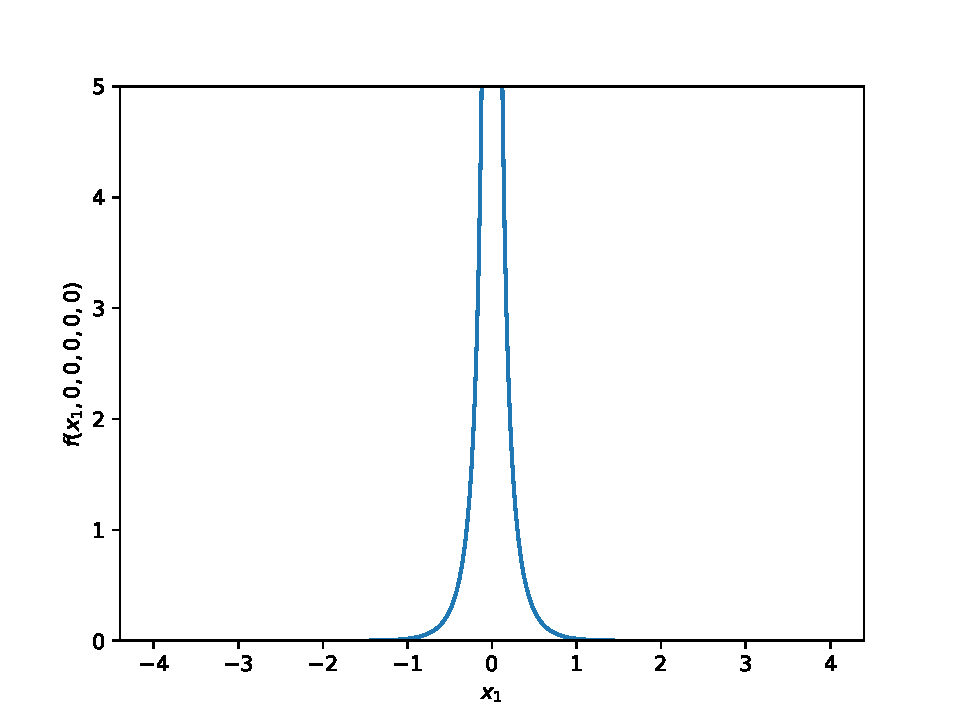
\includegraphics[width=11cm]{Function.pdf}
\caption[Plot of function]{Plot of the integrand as a function of $x_1$ when $x_2=y_1=y_2=z_1=z_2=0$.}
\end{figure}
The integration limit is then changed to $[-2,2]$ for all 6 integrands. It is then possible to map the Legendre functions from $[-1,1]$ to $[-2,2]$. Because any of the 6 variables in the integral are freely interchangeable, the approximation then reads,
$$\int_{-\infty}^{\infty}\int_{-\infty}^{\infty}\int_{-\infty}^{\infty}\int_{-\infty}^{\infty}\int_{-\infty}^{\infty}\int_{-\infty}^{\infty}f(x_1,x_2,y_1,y_2,z_1,z_2)dx_1dx_2dy_1dy_2dz_1dz_2$$
$$\approx\int_{-2}^{2}\int_{-2}^{2}\int_{-2}^{2}\int_{-2}^{2}\int_{-2}^{2}\int_{-2}^{2}f(x_1,x_2,y_1,y_2,z_1,z_2)dx_1dx_2dy_1dy_2dz_1dz_2 $$
$$\approx\sum_{i=1}^{N}\sum_{j=1}^{N}\sum_{k=1}^{N}\sum_{l=1}^{N}\sum_{m=1}^{N}\sum_{n=1}^{N}\omega_i\omega_j\omega_k\omega_l\omega_m\omega_nf(x_i,x_j,x_k,x_l,x_m,x_n)$$
where $x_i$ and $\omega_i$ are the weights and the mesh points from the Gauss- Legendre quadrature.
This will lead to a total of $N^6$ function evaluations. A possible problem to face is that one will end up dividing by zero $N^3$ times. This problem can be faced by ignoring all function evaluations where the function's denominator is lower than a threshold, which was chosen to be $10^{-8}$.
\subsubsection{Laguerre and Legendre polynomials}
When transferred into spherical coordinates, the integral reads

$$
\int_
{0}^{\pi}\int_{0}^{\pi}\int_{0}^{2\pi}\int_{0}^{2\pi}\int_{0}^{\infty}\int_{0}^{\infty}
\frac{r_1^2r_2^2sin(\theta_1)sin(\theta_2)e^{-4(r_1+r_2)}}{\sqrt{r_1^2+r_2^2-2r_1r_2cos(\beta)}}dr_1dr_2d\phi_1d\phi_2d\theta_1d\theta_2
$$
with
$$
cos(\beta)=cos(\theta_1)cos(\theta_2)+sin(\theta_1)sin(\theta_2)cos(\phi_1-\phi_2)
$$

This has the advantage that infinity only has to be faced twice, and Laguerre-Polynomials can be used for that. Laguerre-polynomials are defined for $[0,\infty)$ and have a weight function $W(x)=e^{-x}$. This is relevant for $r_1$ and $r_2$, as the integration limits go from $0$ to $\infty$. The angles $\theta_1$ and $\theta_2$ lie in $[0,\pi]$, and the angles $\phi_1$ and $\phi_2$  lie in $[0,2\pi]$. Here, Lagrange-Polynomials can be used again. Because each of the $\theta$, $\phi$ and $r$ are interchangeable, it is necessary to create 3 types of mesh points and weights: One using the Laguerre polynomials  ($\omega_r$, $x_r$), one using Lagrange polynomials for the angle $\theta$ ($\omega_\theta$, $x_\theta$) and one using Lagrange polynomials for the angle $\phi$ ($\omega_\phi$, $x_\phi$). The function to be evaluated changes slightly due to the Laguerre-polynomials weight function, the exponent goes from -4 to -3, leading to
$$g(r_1,r_2,\theta_1,\theta_2,\phi_1,\phi_2)=\frac{r_1^2r_2^2sin(\theta_1)sin(\theta_2)e^{-3(r_1+r_2)}}{\sqrt{r_1^2+r_2^2-2r_1r_2cos(\beta)}}$$
$$\int_{0}^{\pi}\int_{0}^{\pi}\int_{0}^{2\pi}\int_{0}^{2\pi}\int_{0}^{\infty}\int_{0}^{\infty}
g(r_1,r_2,\theta_1,\theta_2,\phi_1,\phi_2)dr_1dr_2d\phi_1d\phi_2d\theta_1d\theta_2$$
This integral is then approximated by the following sum:

$$
\approx \sum_{i=1}^N \sum_{j=1}^N \sum_{k=1}^N \sum_{l=1}^N \sum_{m=1}^N \sum_{n=1}^N \omega_{r,i} \omega_{r,j} \omega_{\theta ,k} \omega_{\theta ,l} \omega_{\phi ,m} \omega_{\phi ,n} g(x_{r,i},x_{r,j},x_{\theta ,k},x_{\theta ,l},x_{\phi ,m},x_{\phi ,n})
$$
Again, the risk of dividing by zero is averted when the denominator  is lower than a threshold, which was chosen to be $10^{-8}.$
\subsubsection{Monte Carlo integration without importance sampling}
The first approach is to use Monte Carlo with uniformly distributed values for each dimension in the range $[-\lambda,\lambda]$, as no uniform distributions for $(-\infty,\infty)$ exist. As for the Lagrange polynomials, the integration limits were changed  to $[-2,2]$ for all 6 integrands. Using the PDF p(x)=0.25 for $x\in [-2,2]$, otherwise zero, the integral reads 
$$\int_{-2}^{2}\int_{-2}^{2}\int_{-2}^{2}\int_{-2}^{2}\int_{-2}^{2}\int_{-2}^{2}0.25^64^6f(x_1,x_2,y_1,y_2,z_1,z_2)dx_1dx_2dy_1dy_2dz_1dz_2$$
$$\approx4^6\frac{1}{N}\sum_{i=1}^{N}f(x_{i,1},x_{i,2},x_{i,3},x_{i,4},x_{i,5},x_{i,6})$$
where $x_{i,1},...,x_
{i,6}$ are uniformly distributed in  [-2,2]. Again, all function evaluations where the denominator is smaller than $10^{-8}$, are ignored.
\subsubsection{Monte Carlo integration with importance sampling}
In polar coordinates, the polar part of the function resembles the PDF $p(r_1,r_2)=16e^{-4(r_1+r_2)}$, where $p(r_1,r_2)$ is the product of two exponential distributions with parameter=4. Thus, it is possible to sample both $r_1$ and $r_2$ from that exponential distribution.
The angles $\theta_1$ and $\theta_2$ can be sampled from a uniform distribution for values in $[0,\pi]$, while the angles  $\phi_1$ and $\phi_2$ are taken from a uniform distribution for values in $[0,2\pi]$. Doing this, the function that we want to get the expectation value from is given by
$$g(r_1,r_2,\theta_1,\theta_2,\phi_1,\phi_2)=\pi^4\frac{2^2}{4^2}\frac{r_1^2r_2^2sin(\theta_1)sin(\theta_2)}{\sqrt{r_1^2+r_2^2-2r_1r_2cos(\beta)}}$$
with $cos(\beta)$ as defined earlier.
Thus, the integral is approximated by
$$\frac{1}{N}\sum_{i=1}^{N}g(r_{i,1},r_{i,2},\theta_{i,1},\theta_{i,2},\phi_{i,1},\phi_{i,2})$$
where $r_{i,1},r_{i,2}$ are exponentially distributed with a factor 4;  $\theta_{i,1},\theta_{i,2}$ are uniformly distributed in $[0,\pi]$, and  $\phi_{i,1},\phi_{i,2}$  are uniformly distributed in $[0,2\pi]$. In order to create exponentially distributed random variables, we use that a variable $x_i$ is exponentially distributed when
$$x_i=-\frac{1}{4}ln(1-u_i)$$
where $u_i$ is standard uniformly distributed. Again, all function evaluations where the denominator is smaller than $10^{-8}$, are ignored.
\subsection{Computational implementation}
The computational implementation of the formulas that were found was rather straightforward. For the Legendre polynomials, Numerical Recipe's ${\textit{gauleg}}$ function was used to fill to arrays of size N with the mesh points and weights, for the Laguerre polynomials, we used Numerical Recipe's ${\textit{gaulag}}$ function \cite{press1992numerical}. The 6-fold sums were then implemented as 6-fold loops.\\
For the Monte Carlo integration, we used the Mersenne Twister random number generator to create standard uniformly distributed numbers and transformed them according to the earlier described process. We tested both the Laguerre polynomials, the Lagrange polynomials and Monte Carlo integration on example integrals to make sure that everything works as predicted. We then used Python scripts to analyse and plot the data we have gotten.
\subsubsection{Parallelization}
Because each of the 4 approaches calculates terms in a sum that are independent of each other, it is easy to parallelize the code. We made a parallelized version of each of the 4 approaches as well. The code was parallelized using MPI, and a flexible function was created by us to make sure that each thread gets the same amount of workload. The 6-fold for loops used in the Gaussian quadrature were replaced by a single while-loop with multiple if-else clauses that essentially do the same.

\section{Results}
\subsection{Legendre polynomials}
The results achieved using Legendre polynomials with a cutoff $\lambda=2$, as well as time use for both the parallelized and the non-parallelized case, and the deviation from the correct result, can be found in table 1.

\begin{table}[H]
\caption[Cartesian Quadrature using Legendre polynomials]{Achieved results, relative error, time-usage in seconds (averaged over 5 simulations, but for n=55 and n=65)for both the nonparallel and the parallel program (without optimization flags) as well as standard error for integration using Legendre polynomials. }
\begin{tabular}{|l|l|l|l|l|}
\hline
N          & Result   & Relative Error & \pbox{10cm}{time {[}s{]}\\ parallelized}  &  \pbox{10cm}{time {[}s{]}\\ nonparallelized} \\ \hline
10 & 0.129834 & 0.326466       & 0.021025232                             & 0.0388234 \\ \hline
15 & 0.199475 & 0.0348043      & 0.1436784                               & 0.4376558 \\ \hline
20 & 0.177065 & 0.0814488      & 0.7488488                               & 2.70073   \\ \hline
25 & 0.189110  & 0.018967       & 3.107388                                & -       \\ \hline
30 & 0.185796 & 0.0361583      & 8.855728                                & 29.37128  \\ \hline
40 & 0.18867  & 0.0212464      & 49.99648                                & -       \\ \hline
45 & 0.190128 & 0.0136823      & 95.06266                                & -       \\ \hline
55 & 0.190669 & 0.0108763      & 303.598                                 & -       \\ \hline
65 & 0.191035 & 0.00897612     & 823.381                                 & -       \\ \hline
\end{tabular}
\end{table}

Even though the relative error tends to get smaller for larger values of N, even with N=65, there is a divergence between the analytical and the numerical result. Choosing a different threshold $\lambda$ might improve the result, as would larger values of N. One interesting aspect is that, for specific values of N ($N=15$, $N=25$), one gets more correct results than for larger values of n. This is presumably caused by us ending up getting "lucky" mesh points and weights. However, none of the results give close results, and the error is in the third decimal.
\subsection{Laguerre and Legendre polynomials}

The results achieved using Laguerre Polynomials for the radial parts and Legendre polynomials for the angle parts of the spherical integral as well as time use for both the parallelized and the nonparallelized case, and the deviation from the correct result, can be found in table 2.

\begin{table}[H]
\caption[Spherical Quadrature using Laguerre polynomials]{Achieved results, relative error, time-usage in seconds (averaged over 5 simulations, but for n=55 and n=65)for both the nonparallel and the parallel program (without optimization flags) as well as standard error for integration using Laguerre polynomials (for the radial parts).}
\begin{tabular}{|l|l|l|l|l|}
\hline
N         & Result   & Relative Error & \pbox{10cm}{time {[}s{]}\\ parallelized}  &  \pbox{10cm}{time {[}s{]}\\ nonparallelized} \\ \hline
10 & 0.177081 & 0.0813679      & 0.05331922                              & 0.1115982 \\ \hline
15 & 0.193285 & 0.00269565     & 0.3914072                               & 1.200048  \\ \hline
20 & 0.194786 & 0.0104784      & 2.044996                                & 7.023426  \\ \hline
25 & 0.194804 & 0.0105751      & 8.18345                                 & -       \\ \hline
30 & 0.194779 & 0.010443       & 25.8677                                 & 81.0227   \\ \hline
40 & 0.194669 & 0.009873       & 142.9906                                & -       \\ \hline
45 & 0.194594 & 0.00948246     & 269.7448                                & -       \\ \hline
55 & 0.194439 & 0.00868232     & 884.532                                 & -       \\ \hline
65 & 0.194298 & 0.00794811     & 2429.59                                 & -       \\ \hline
\end{tabular}
\end{table}

Compared to the Cartesian Legendre polynomials case, even quite small values of N give good estimates for the total result. However, for larger values of N, we did not achieve much better results than with using Legendre polynomials, which is surprising, given that the correct integration limits are taken into account. It is also quite interesting to see that evaluating the Laguerre polynomials takes roughly 3 times as much time as the Legendre polynomials. This might be caused by the computer system having to look up in different arrays, or by the more complex function that is evaluated. Again,for $N=15$, one gets a surprisingly correct result, which is presumably caused by lucky mesh points.
\subsection{Cartesian Monte Carlo without importance sampling}
The results achieved using Monte Carlo simulation and uniform distributions for Cartesian coordinates as well as time use for both the parallelized and the nonparallelized case, and the deviation from the correct result and the standard error $\sigma^2/\sqrt{N}$, can be found in table 3.

\begin{table}[H]
\caption[Cartesian Monte Carlo without importance sampling]{Achieved results, relative error, time-usage in seconds (averaged over 5 simulations) for both the nonparallel and the parallel program (without optimization flags) as well as standard error for different values of N for Cartesian Monte Carlo without importance sampling. The result with the median relative error is presented, the standard error is calculated from the averaged variance over 5 runs.}
\begin{tabular}{|l|l|l|l|l|l|}
\hline
N          & Result   & Relative Error & \pbox{10cm}{time {[}s{]}\\ parallelized}  &  \pbox{10cm}{time {[}s{]}\\ nonparallelized} &  \pbox{10cm}{Standard\\ Error} \\ \hline
$10^3$ & 0.122134 & 0.366414   & 0.0003482432 & 0.0003056 & 0.1344    \\ \hline
$10^4$ & 0.140808 & 0.269539   & 0.002769808  & 0.0034032 & 0.2318    \\ \hline
$10^5$ & 0.20568  & 0.066995   & 0.02500496   & 0.0328912 & 0.02865   \\ \hline
$10^6$ & 0.183756 & 0.046738   & 0.10475636   & 0.3262482 & 0.008598  \\ \hline
$10^7$ & 0.191025 & 0.00902881 & 0.8515582    & 3.090702  & 0.006693  \\ \hline
$10^8$ & 0.192471 & 0.00152991 & 8.520786     & 29.38188  & 0.0009739 \\ \hline
$10^9$ & 0.192261 & 0.00261722 & 91.32978     & -         & 0.0003159 \\ \hline
\end{tabular}
\end{table}

As expected, larger values of N lead to more correct results, and the standard error goes down (but for $N=10^4$, where the result is completely off. However, this only happened for one of the 5 simulations).
Compared to the Legendre polynomials, that solve exactly the same integral, the results are closer to the real result. However, the result for for $N=10^9$, which is $0.192261$, is more than one standard error smaller than the analytical solution, which can give the wrong impression that this wrong result indeed is correct. This is due to the fact that parts of the integral are omitted. Choosing a larger threshold value $\lambda$ would likely lead to a more correct result, but we did not test this further. 
\subsection{Spherical Monte Carlo with importance sampling}
The results achieved using Monte Carlo simulation with importance sampling as described earlier in spherical coordinates as well as time use for both the parallelized and the nonparallelized case, and the deviation from the correct result and the standard error $\sigma^2/\sqrt{N}$, can be found in table 4.

\begin{table}[H]
\caption[Spherical Monte Carlo with importance sampling]{Achieved results, relative error, time-usage in seconds (averaged over 5 simulations) for both the nonparallel and the parallel program (without optimization flags) as well as standard error for Cartesian Monte Carlo with importance sampling.  The result with the median relative error is presented, the standard error is calculated from the averaged variance over 5 runs.}
\begin{tabular}{|l|l|l|l|l|l|}
\hline
N          & Result   & Relative Error & \pbox{10cm}{time {[}s{]}\\ parallelized}  &  \pbox{10cm}{time {[}s{]}\\ nonparallelized} &  \pbox{10cm}{Standard\\ Error} \\ \hline
$10^3$       & 0.220074 & 0.141665    & 0.0005288586 & 0.0004486 & 0.05248   \\\hline
$10^4$      & 0.197875 & 0.0265038   & 0.00493595   & 0.0048254 & 0.009458  \\\hline
$10^5$     & 0.195131 & 0.0122716   & 0.03278686   & 0.0480236 & 0.003511  \\\hline
$10^6$    & 0.192313 & 0.00234779  & 0.158712     & 0.4711302 & 0.001036  \\\hline
$10^7$   & 0.193096 & 0.00171425  & 1.236776     & 4.575088  & 0.0003362 \\\hline
$10^8$  & 0.192688 & 0.000403855 & 13.06474     & 42.41482  & 0.0001037 \\\hline
$10^9$ & 0.192784 & 9.70237E-05 & 141.535      & -       & 3.287$\cdot10^{-5}$\\\hline
\end{tabular}
\end{table}

As expected, increasing N leads to more correct results. Compared to the other methods, this method leads to the most correct result, and we ended up having $0.192784\pm 3.287\cdot10^{-5}$ as our final result.Even for comparatively small values of N, such as $N=10^7$, the achieved result is closer to the analytical solution, and for  $N=10^9$, the standard error is in the magnitude of $N=10^{-5}$, with a result that is close enough to the analytical solution to be used further.
\subsection{Time usage and parallelization}
Figure 2 plots the relative error (in log-scale) of the different algorithms against the time use (in log-scale) for the parallelized algorithms.
\begin{figure}[H]
\centering
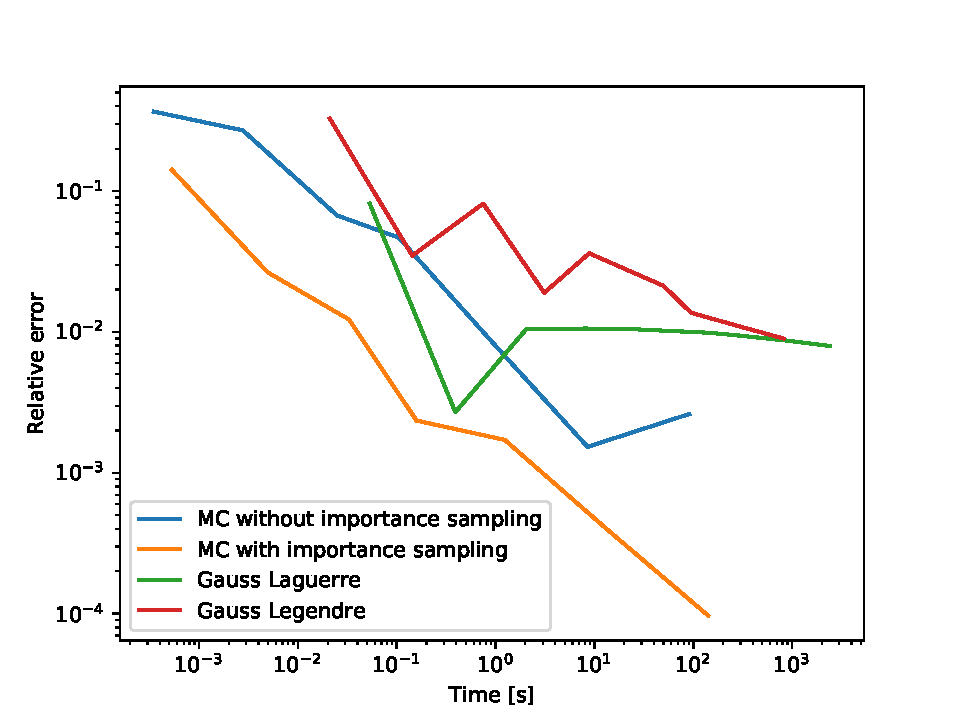
\includegraphics[width=11cm]{Error_time_use.pdf}
\caption[Time vs. relative error]{Time usage [s] of parallelized algorithms plotted against the methods' relative error. Logarithmic scales for both axes were used. The data from the tables 1-4 was used.}\label{Error_time_use}
\end{figure}
This graph clearly shows that both Monte Carlo approaches lead to better results than the Gaussian quadrature methods, but for the "lucky" result in the Laguerre results. It also shows that clever importance sampling can further decrease the relative error in a magnitude of almost $10^{-2}$, compared to the  other Monte Carlo approach. It also gives the impression that neither of the quadrature approaches would lead to much better results, even upon increasing N, while the Monte Carlo methods, especially the one with importance sampling, could decrease the error even further. It should be mentioned that a possible reason why the Monte Carlo approach without importance sampling gives a worse result for it's most time consuming calculation (with $N=10^9$), might be due to the way the represented value was chosen - the median value. \\\\
Figure 3 plots the value N against the relative difference in time use when the nonparallelized algorithm is compared to the parallelized algorithm for the Monte Carlo case with importance sampling.
\begin{figure}[H]
\centering
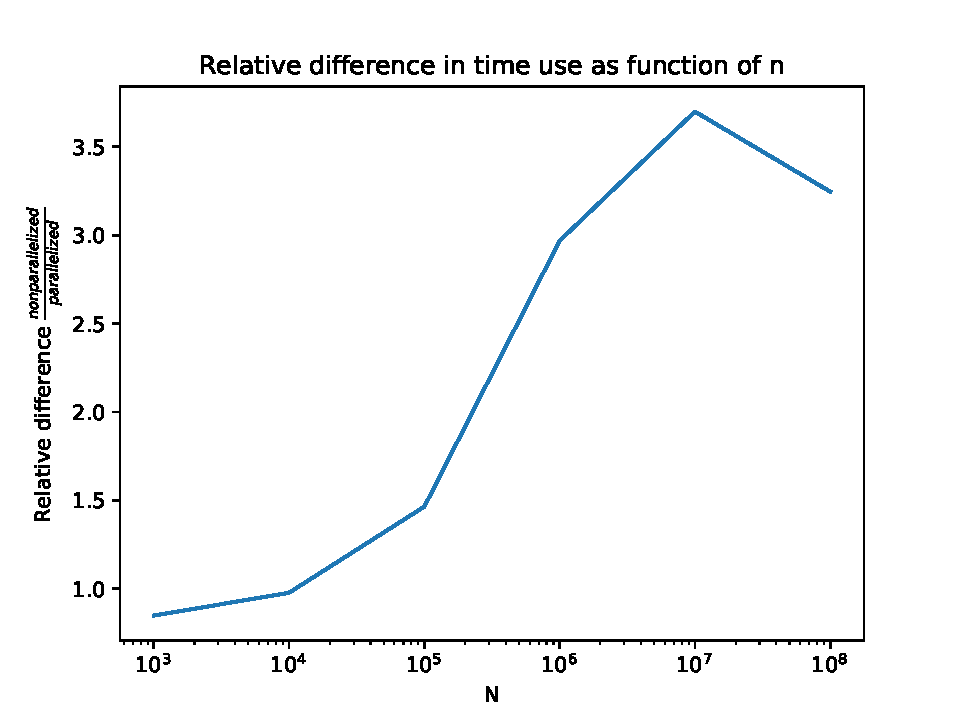
\includegraphics[width=11cm]{Relative_difference_time.pdf}
\caption[N vs. relative time use]{N (logarithmic scale) plotted against the relative difference in time use between the nonparallelized and the parallelized algorithm. Data from table 4 was used.}\label{N vs. relative time use}
\end{figure}
One can clearly see how parallelization, or at least the way we implemented it, does not give faster results for small values of N. To the contrary, for N up to $10^4$, parallelization increases the average run time. However, for larger values of N, such as $10^8$, parallelization makes the program run 3 to 3.5 times faster. This is less than theoretically possible (one could get a boost of up to 4 on 4 identical CPU cores), but still clearly justifies the process of parallelizing a program, especially when the run times are large. The other 3 approaches gave similar results, as can be seen in tables 1-3. The reason why no perfect time enhancement was achieved probably lies in an imperfect implementation, as each process has to run some functions, that in theory do not need to be re-run several times, and in that only the time-sensitive parts are parallelized.\\\\
We also tested the impact of the "-O3" parallelization flag on the run time. The results can be seen in figure 4:
\begin{figure}[H]
\centering
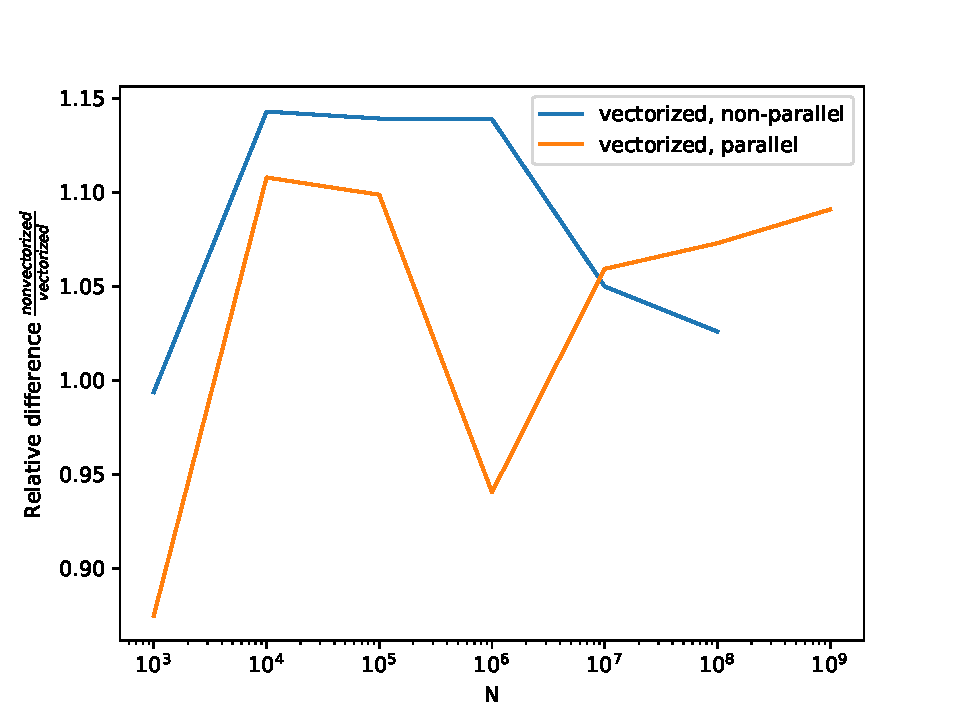
\includegraphics[width=11cm]{Parrallelisation_flag.pdf}
\caption[Vectorization flags]{N (logarithmic scale) plotted against the relative difference in time use between the non-vectorized and the vectorized program. }
\end{figure}
The "-O3"-flag seems to have a small, but not negligible impact on the run time of both the parallelized and the non-parallelized code, and for large N, the compiler flag seems to give an additional speed boost.
However, that behaviour is quite erratic, and the time improvement is very small, making this data not completely reliable. It is possible that careful coding of loops could improve these results.
\section{Conclusion}
The application of Gauss- Legendre quadrature was for this particular integral, a poor choice. In this instance, errors were introduced at several points. When approximating the function value of the integrand to be zero at inputs greater that 2, and when approximating the function by a polynomial of degree $2N-1$.\\Instead, by using the more appropriate choice of the Gauss- Laguerre quadrature, for the two radial variables; those ranging from zero to infinity and Gauss- Legendre for the remaining variables through a change of variables. Errors are only introduced in approximating the function values with that of polynomials of degree $2N-1$.\\\\Monte- Carlo integration is an excellent choice for six- dimensional integrals and higher, as the error scales with $\frac{1}{\sqrt{N}}$ for a number of mesh points $N$ regardless of the dimensionality of the integral. The choice of whether or not to tailor the PDF to suit the integrand, proved to have a tremendous effect on the time expenditure and accuracy of the program, with importance sampling accounting for an approximately  $97\%$ decrease in relative error, measured at $N = 10^9$ mesh points. See appendix(\ref{Monte- Carlo relative error improvement}), but also an approximately $55\%$ increase in time expenditure (measured for the parallelized programs at $N = 10^9$. See appendix (\ref{Monte- Carlo time increase}).\\\\The implementation of parallelization proved to be especially worth while for $N>10^5$ as is seen in figure \ref{N vs. relative time use}. The speed up should on the surface be 4 times greater on computers with quad- core computer chips, however factors such as writing and fetching to and from memory impacts this effect negatively, especially when moving from fast to slow memory. The effect could still be primarily because of a potentially non- optimal implementation of parallelization flags.
\section{Appendix}
\subsection{Proof that \textbf{L} is invertible}\label{Proof that big ass matrix is invertible}
For the matrix $\textbf{L}$ in equation \ref{Big ass matrix}; each column is constructed of constants multiplied with the Laguerre polynomial $L_n$ for each row in column $n$. With the Laguerre polynomials being orthogonal with respect to the inner product
\begin{equation}
\braket{L_n|L_m} = \int\limits_0^\infty  e^{-x} L_n(x) L_m(x) dx = \delta_{mn}
\end{equation}
no column can be expressed as a linear combination of any of the others (at least not for $x \in [0,\infty]$, so \textbf{L} is an $N\times N$ matrix with $N$ linearly independent columns. As such it is necessarily non-singular and therefore, must be invertible.
\subsection{Proof that $F^{-1}(U)$ has cumulative function F(x)}
Let F(X) be a cumulative distribution function (CDF).\\
Let U be standard uniformly distributed and let G be it's CDF, that is, $G(u)=u$ for $0\leq u\leq 1$, otherwise 0.\\
Assume that $X=F^{-1}(U)$. Then
$$F(x)=P(X\leq x)=P(F^{-1}(U)\leq x)=P(U\leq F(x))=G(F(x))=F(x) 
$$ 
\subsection{Monte- Carlo relative error improvement with importance sampling}\label{Monte- Carlo relative error improvement}
Relative error in the Monte- Carlo method with and without importance sampling at $N = 10^9$
$$
\frac{0.00261722-0.0000970237}{0.00261722}\cdot 100 \approx 96.3\%.
$$
The absolute error decreased by approximately $96.3\%$ when implementing importance sampling at $N = 10^9$.
\subsection{Monte- Carlo time expenditure increase with importance sampling}\label{Monte- Carlo time increase}
The increased time expenditure for Monte- Carlo with importance sampling at $N = 10^9$
$$
\frac{141.535-91.330}{91.330}\cdot 100 \approx 55\%.
$$
The time expenditure increased by approximately $55\%$ when implementing importance sampling at $N = 10^9$.
\subsection{List of programs}
All programs can be found on \url{https://github.com/adrian2208/FYS3150_collab} in the folder "project 3".


\begin{itemize}
\item[1.] a.cpp - Legendre approach to solve the integral
\item[2.] b.cpp - Legendre and Laguerre approach to solve the integral
\item[3.] c.cpp - Monte Carlo approach (no importance sampling) to solve the integral
\item[4.] d.cpp - Monte Carlo approach (with importance sampling)  approach to solve the integral
\item[5.] a\_parallel.cpp - Parallelized version of a.cpp
\item[6.] b\_parallel.cpp - Parallelized version of b.cpp
\item[7.] c\_parallel.cpp - Parallelized version of c.cpp
\item[8.] d\_parallel.cpp - Parallelized version of d.cpp
\item[9.] testings.cpp - Unit testing.
\item[10.] tests\_main.cpp - Unit testing.
\item[11.] functions.hpp \& functions.cpp - Contains functions for parallelization, and all the integrands, and some more.
\item[12.] compile\_and\_run.py - Compiles and runs (for many values of n, 5 times with and 5 times without vectorization flags) all files. Also runs testings once.
\item[13.] create\_final\_lists.py - Creates data that was used for tables 1-4 from the raw data. Should be run after compile\_and\_run.py.
\item[14.] databehandling.py - Creates plots from data created by create\_final\_lists.py.
\item[15.] plot\_function.py - Plots the function.
\end{itemize}

\bibliographystyle{Plain}
\bibliography{citations}

\end{document}